\documentclass[12pt, a4paper]{article}
\usepackage[
a4paper,
mag=1000,
left=3cm,
right=1.0cm,
top=2cm,
bottom=2cm,
headsep=0.7cm,
footskip=1cm
]{geometry}
\usepackage[T2A]{fontenc}
\usepackage[utf8]{inputenc}
\usepackage[english,russian]{babel}
\usepackage[colorlinks=true, citecolor=blue, urlcolor=blue, linkcolor=blue]{hyperref}
\usepackage{graphicx}
\usepackage{physics}
\usepackage{amsmath,amssymb}
\usepackage{indentfirst}
\usepackage{float}
\usepackage{multirow}
\usepackage{hhline}
\usepackage{pgfplots}
\pgfplotsset{compat=1.18}
\usepackage{bigstrut}
\usepackage{fancyhdr}
\usepackage{caption}
\usepackage{setspace}
\usepackage{array}

\DeclareCaptionLabelSeparator{dash}{ -- }
\captionsetup{labelsep=dash}
\captionsetup[table]{justification=raggedright,singlelinecheck=false}

\fancyhf{}
\fancyfoot[C]{Ярославль, 2026}
\renewcommand{\headrulewidth}{0pt}

\begin{document}
	\onehalfspacing
	\thispagestyle{fancy}
	
	\begin{center}
		МИНОБРНАУКИ РОССИИ\\
		Федеральное государственное бюджетное образовательное учреждение высшего образования\\
		«Ярославский государственный университет им. П.Г. Демидова»\\[3mm]
		Кафедра микроэлектроники и общей физики
	\end{center}
	
	\vspace{55mm}
	
	\begin{center}
		Лабораторная работа № 1\\[3mm]
		\textbf{«Исследование движения электронов в электрических и магнитных полях с помощью трубки Томсона»}
	\end{center}
	
	\vspace{20mm}
	
	\begin{flushright}
		Студенты группы ЭН-31БО:\\
		Р.Д. Рахимов, И.И. Ушкало\\[5mm]
		Научный руководитель:\\
		ст. преподаватель\\
		А.Н. Сергеев
	\end{flushright}
	
	\newpage
	
	\section{Цель работы.}
	Изучить движение электрона в электрическом и магнитном полях и определить удельный заряд электрона $e/m$ по отклонению пучка в магнитном поле и методом компенсации отклонений электронного пучка.
	
	\section{Перечень используемого оборудования и материалов.}
	- трубка Томсона S U18555 (анодное напряжение $2000$--$5000$ В, напряжение на пластинах отклоняющего конденсатора не более $350$ В, расстояние между пластинами $d = 8$ мм, размер люминесцентного экрана $80 \times 80$ мм),
	
	- держатель электровакуумных приборов S U185002,
	
	- пара катушек Гельмгольца U185051 (число витков $n = 320$, диаметр катушки $138$ мм, максимально допустимый ток $1$ А, сопротивление одной катушки $6{,}5$ Ом),
	
	- высоковольтный источник питания U33010-230 ($0$--$5000$ В, $0{,}2$ мА, накальный канал $6{,}3$ В),
	
	- многоканальный источник питания постоянного тока U33000-230 (каналы $0$--$500$ В, $0$--$50$ В, $0$--$8$ В, $0$--$12$ В),
	
	- набор безопасных соединительных проводов U138021.
	
	\section{Основные теоретические сведения и расчётные формулы.}
	
	В трубке Томсона электроны испускаются катодом за счёт термоэлектронной эмиссии и ускоряются анодным напряжением $U_A$, приобретая энергию
	\begin{equation}
		\frac{mv^2}{2} = eU_A,
		\label{eq:energy}
	\end{equation}
	откуда скорость электрона
	\begin{equation}
		v = \sqrt{2U_A\,\frac{e}{m}},
		\label{eq:v}
	\end{equation}
	где $e/m$ --- удельный заряд электрона.
	
	\textbf{Движение в электрическом поле.} Напряжённость поля плоского конденсатора $E = U_P/d$, где $U_P$ --- напряжение на пластинах, $d$ --- расстояние между ними. Электрон, влетающий в конденсатор вдоль оси $X$ со скоростью $v$, движется с ускорением $a = eE/m$ по оси $Y$:
	\begin{equation}
		x = vt, \qquad y = \frac{at^2}{2} = \frac{1}{2}\,\frac{e}{m}\,\frac{E}{v^2}\,x^2.
		\label{eq:y}
	\end{equation}
	Подставляя \eqref{eq:v}, получаем, что отклонение не зависит от $e/m$:
	\begin{equation}
		y = \frac{E\,x^2}{4U_A} = \frac{U_P\,x^2}{4dU_A},
		\label{eq:ytheor}
	\end{equation}
	то есть $y$ линейно растёт с $U_P$ и обратно пропорционально $U_A$.
	
	Координаты $x$ и $y$ точки выхода пучка на край экрана находят по шкале (рис.~\ref{fig:geom}): если пучок пересекает шкалу в точке со значением $g$, то
	\begin{equation}
		y = \frac{g}{\sqrt{2}}, \qquad x = \sqrt{2}\,k - y,
		\label{eq:xy}
	\end{equation}
	где $k = 80$ мм --- сторона экрана.
	
	\textbf{Движение в магнитном поле.} На электрон, движущийся в магнитном поле $\vec B$, действует сила Лоренца $\vec F = -e[\vec v \times \vec B]$. Так как $\vec v \perp \vec B$, она играет роль центростремительной силы:
	\begin{equation}
		Bev = \frac{mv^2}{r}.
		\label{eq:lorentz}
	\end{equation}
	Из \eqref{eq:v} и \eqref{eq:lorentz} получаем удельный заряд
	\begin{equation}
		\frac{e}{m} = \frac{2U_A}{(Br)^2}.
		\label{eq:em}
	\end{equation}
	Индукция магнитного поля катушек Гельмгольца
	\begin{equation}
		B = \left(\frac{4}{5}\right)^{3/2}\frac{\mu_0 n}{R}\,I = kI, \qquad k = 4{,}2\ \frac{\text{мТл}}{\text{А}},
		\label{eq:B}
	\end{equation}
	где $\mu_0$ --- магнитная постоянная, $R$ --- средний радиус катушки, $n$ --- число витков, $I$ --- ток в катушках. При отсутствии амперметра ток находят по закону Ома: катушки сопротивлением $6{,}5$ Ом соединены параллельно, их общее сопротивление $3{,}25$ Ом, поэтому $I = U/3{,}25$.
	
	Радиус траектории $r$ находят по точке $A$ выхода пучка на шкалу (рис.~\ref{fig:geom}): $r = (c^2 + a^2)/(2a)$, откуда при $k = 80$ мм
	\begin{equation}
		r = \frac{(80\ \text{мм})^2 + h^2}{\sqrt{2}\,(80\ \text{мм} - h)}, \qquad h = 80\ \text{мм} - g.
		\label{eq:r}
	\end{equation}
	
	\textbf{Метод компенсации.} Если электрическое и магнитное поля подобраны так, что отклонение пучка компенсируется (пучок идёт по оси трубки к дальнему углу экрана), то
	\begin{equation}
		eE = evB, \qquad v = \frac{E}{B}.
		\label{eq:comp}
	\end{equation}
	С учётом \eqref{eq:v}
	\begin{equation}
		\frac{e}{m} = \frac{1}{2U_A}\left(\frac{E}{B}\right)^2.
		\label{eq:emcomp}
	\end{equation}
	На этом основан фильтр скоростей: через область скрещённых полей без отклонения проходят только частицы со скоростью $v = E/B$.
	
	\newpage
	Среднее значение и относительная погрешность относительно табличного значения $(e/m)_0 = 1{,}7588 \cdot 10^{11}$ Кл/кг:
	\begin{equation}
		\left(\frac{e}{m}\right)_{\text{ср}} = \frac{1}{N}\sum_{i=1}^{N}\left(\frac{e}{m}\right)_i, \qquad
		\delta = \frac{\left|(e/m)_{\text{ср}} - (e/m)_0\right|}{(e/m)_0}\cdot 100\%.
		\label{eq:delta}
	\end{equation}
	
	\section{Схема лабораторной установки.}
	\begin{figure}[H]
		\centering
		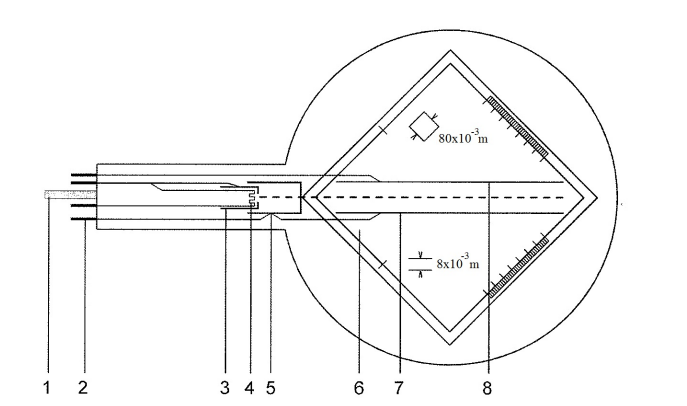
\includegraphics[width=11cm]{tube}
		\caption{Устройство трубки Томсона: 1 --- ключ, 2 --- контактные штырьки, 3 --- катод, 4 --- нагреватель катода, 5 --- анод, 6 --- флюоресцентный экран, 7 и 8 --- отклоняющие пластины}
		\label{fig:tube}
	\end{figure}
	
	
	\section{Порядок выполнения работы.}
	\begin{enumerate}
		\item Собрана установка по схеме (рис.~\ref{fig:wiring}): регуляторы блоков питания выведены на минимум (против часовой стрелки до упора), пластины конденсатора подключены к выходу $0$--$500$ В, катушки Гельмгольца --- к выходу $0$--$12$ В.
		\item Включён высоковольтный блок питания, подано напряжение накала катода.
		\item \textit{Упражнение 1.} При анодном напряжении $U_A = 2000$ В изменялось напряжение на пластинах конденсатора $U_P$ (не более $350$ В) с шагом $50$ В от $50$ до $300$ В; на экране определено значение $g$ в точке пересечения пучка со шкалой и по формулам \eqref{eq:xy} найдены $x$ и $y$. Построена зависимость $y(U_P)$. Опыт повторён при $U_A = 3000$ В и $4000$ В.
		\item \textit{Упражнение 2.} Напряжение на конденсаторе установлено равным нулю, при $U_A = 2000$, $3000$ и $4000$ В через катушки Гельмгольца пропущен ток $I = 0{,}5$; $0{,}6$ и $0{,}7$ А (не более $1$ А). По положению пучка определены $g$, $h$, радиус траектории $r$ по формуле \eqref{eq:r}, а удельный заряд электрона --- по формуле \eqref{eq:em}.
		\newpage
		\item \textit{Упражнение 3.} При заданных $U_A$ и $I$ напряжением $U_P$ (не более $350$ В) достигнута компенсация отклонения пучка, по формуле \eqref{eq:emcomp} вычислен удельный заряд электрона. Опыт выполнен при $U_A = 2000$, $3000$, $4000$ В и $I = 0{,}1$; $0{,}2$; $0{,}3$ А; при $U_A = 3000$ и $4000$ В и $I = 0{,}3$ А результат не получен.
		\item \textit{Упражнение 4.} По данным упражнения 3 по формуле \eqref{eq:comp} определена скорость электронов для каждого опыта.
		\item Найдены среднее значение $e/m$ и относительная погрешность по формуле \eqref{eq:delta}. Все вычисления выполнены в системе СИ.
	\end{enumerate}
	
	\section{Ход выполнения работы.}
	
	\subsection{Упражнение 1. Движение электронов в электрическом поле.}
	Результаты измерений приведены в табл.~\ref{tab:ex1}. Теоретическое значение $y_{\text{теор}}$ рассчитано по формуле \eqref{eq:ytheor} при $d = 8$ мм.
	
	\begin{table}[H]
		\caption{Отклонение электронного пучка в электрическом поле}
		\label{tab:ex1}
		\centering
		\small
		\begin{tabular}{|c|c|c|c|c|c|}
			\hline
			\multirow{6}{*}{2000} & 50 & 8 & 5,66 & 107,48 & 9,03 \\ \cline{2-6}
			& 100 & 12 & 8,49 & 104,65 & 17,11 \\ \cline{2-6}
			& 150 & 16 & 11,31 & 101,82 & 24,30 \\ \cline{2-6}
			& 200 & 18 & 12,73 & 100,41 & 31,51 \\ \cline{2-6}
			& 250 & 20 & 14,14 & 98,99 & 38,28 \\ \cline{2-6}
			& 300 & 22 & 15,56 & 97,58 & 44,63 \\ \hline
			\multirow{6}{*}{3000} & 50 & 5 & 3,54 & 109,60 & 6,26 \\ \cline{2-6}
			& 100 & 10 & 7,07 & 106,07 & 11,72 \\ \cline{2-6}
			& 150 & 14 & 9,90 & 103,24 & 16,65 \\ \cline{2-6}
			& 200 & 15 & 10,61 & 102,53 & 21,90 \\ \cline{2-6}
			& 250 & 18 & 12,73 & 100,41 & 26,26 \\ \cline{2-6}
			& 300 & 19 & 13,44 & 99,70 & 31,06 \\ \hline
			\multirow{6}{*}{4000} & 50 & 5 & 3,54 & 109,60 & 4,69 \\ \cline{2-6}
			& 100 & 8 & 5,66 & 107,48 & 9,03 \\ \cline{2-6}
			& 150 & 12 & 8,49 & 104,65 & 12,83 \\ \cline{2-6}
			& 200 & 14 & 9,90 & 103,24 & 16,65 \\ \cline{2-6}
			& 250 & 16 & 11,31 & 101,82 & 20,25 \\ \cline{2-6}
			& 300 & 18 & 12,73 & 100,41 & 23,63 \\ \hline
		\end{tabular}
	\end{table}
	
	Пример расчёта для $U_A = 2000$ В, $U_P = 50$ В, $g = 8$ мм:
	\[
	y = \frac{8}{\sqrt{2}} \approx 5{,}66\ \text{мм}, \quad x = \sqrt{2}\cdot 80 - 5{,}66 \approx 107{,}48\ \text{мм}, \quad y_{\text{теор}} = \frac{50\cdot(107{,}48\cdot 10^{-3})^2}{4\cdot 8\cdot 10^{-3}\cdot 2000} \approx 9{,}03\ \text{мм}.
	\]
	
	\begin{figure}[H]
		\centering
		\begin{tikzpicture}
			\begin{axis}[
				width=0.94\textwidth,
				height=8cm,
				xlabel={$U_P$, В},
				ylabel={$y$, мм},
				xmin=0, xmax=320, ymin=0,
				grid=major,
				tick label style={font=\small},
				label style={font=\normalsize},
				legend pos=north west,
				legend style={font=\small},
				]
				\addplot[only marks,mark=*,blue] coordinates {(50,5.657) (100,8.485) (150,11.314) (200,12.728) (250,14.142) (300,15.556)};
				\addlegendentry{$U_A = 2000$ В}
				\addplot[only marks,mark=square*,red!75!black] coordinates {(50,3.536) (100,7.071) (150,9.899) (200,10.607) (250,12.728) (300,13.435)};
				\addlegendentry{$U_A = 3000$ В}
				\addplot[only marks,mark=triangle*,black] coordinates {(50,3.536) (100,5.657) (150,8.485) (200,9.899) (250,11.314) (300,12.728)};
				\addlegendentry{$U_A = 4000$ В}
			\end{axis}
		\end{tikzpicture}
		\caption{Зависимость отклонения пучка $y$ от напряжения на пластинах $U_P$ при разных анодных напряжениях}
		\label{fig:y-up}
	\end{figure}
	
	\subsection{Упражнение 2. Определение $e/m$ по отклонению в магнитном поле.}
	Индукция $B = kI$ при $k = 4{,}2$ мТл/А. Результаты приведены в табл.~\ref{tab:ex2}.
	
	\begin{table}[H]
		\caption{Определение удельного заряда электрона по отклонению в магнитном поле}
		\label{tab:ex2}
		\centering
		\small
		\begin{tabular}{|c|c|c|c|c|c|c|}
			\hline
			\multirow{3}{*}{2000} & 0,5 & 2,10 & 66 & 14 & 70,7 & 1,82 \\ \cline{2-7}
			& 0,6 & 2,52 & 74 & 6 & 61,5 & 1,67 \\ \cline{2-7}
			& 0,7 & 2,94 & 88 & -8 & 51,9 & 1,72 \\ \hline
			\multirow{3}{*}{3000} & 0,5 & 2,10 & 56 & 24 & 88,1 & 1,75 \\ \cline{2-7}
			& 0,6 & 2,52 & 62 & 18 & 76,7 & 1,61 \\ \cline{2-7}
			& 0,7 & 2,94 & 72 & 8 & 63,5 & 1,72 \\ \hline
			\multirow{3}{*}{4000} & 0,5 & 2,10 & 50 & 30 & 103,2 & 1,70 \\ \cline{2-7}
			& 0,6 & 2,52 & 57 & 23 & 86,0 & 1,71 \\ \cline{2-7}
			& 0,7 & 2,94 & 62 & 18 & 76,7 & 1,57 \\ \hline
		\end{tabular}
	\end{table}
	
	Пример расчёта для $U_A = 2000$ В, $I = 0{,}5$ А, $g = 66$ мм ($B = 4{,}2\cdot 0{,}5 = 2{,}10$ мТл):
	\[
	h = 80 - 66 = 14\ \text{мм}, \quad r = \frac{80^2 + 14^2}{\sqrt{2}\,(80 - 14)} \approx 70{,}7\ \text{мм}, \quad \frac{e}{m} = \frac{2\cdot 2000}{(2{,}10\cdot 10^{-3}\cdot 70{,}7\cdot 10^{-3})^2} \approx 1{,}82 \cdot 10^{11}\ \text{Кл/кг}.
	\]
	
	\subsection{Упражнения 3, 4. Метод компенсации и скорость электронов.}
	Результаты приведены в табл.~\ref{tab:ex3}; $E = U_P/d$, скорость $v = E/B$.
	
	\begin{table}[H]
		\caption{Определение $e/m$ методом компенсации и скорость электронов}
		\label{tab:ex3}
		\centering
		\small
		\begin{tabular}{|c|c|c|c|c|c|c|}
			\hline
			\multirow{3}{*}{2000} & 0,1 & 0,42 & 87 & 10,88 & 1,68 & 2,59 \\ \cline{2-7}
			& 0,2 & 0,84 & 181 & 22,62 & 1,81 & 2,69 \\ \cline{2-7}
			& 0,3 & 1,26 & 271 & 33,88 & 1,81 & 2,69 \\ \hline
			\multirow{3}{*}{3000} & 0,1 & 0,42 & 100 & 12,50 & 1,48 & 2,98 \\ \cline{2-7}
			& 0,2 & 0,84 & 229 & 28,62 & 1,94 & 3,41 \\ \cline{2-7}
			& 0,3 & 1,26 & -- & -- & -- & -- \\ \hline
			\multirow{3}{*}{4000} & 0,1 & 0,42 & 114 & 14,25 & 1,44 & 3,39 \\ \cline{2-7}
			& 0,2 & 0,84 & 275 & 34,38 & 2,09 & 4,09 \\ \cline{2-7}
			& 0,3 & 1,26 & -- & -- & -- & -- \\ \hline
		\end{tabular}
	\end{table}
	
	Пример расчёта для $U_A = 2000$ В, $I = 0{,}1$ А, $U_P = 87$ В ($B = 0{,}42$ мТл):
	\[
	E = \frac{87}{8\cdot 10^{-3}} = 1{,}09\cdot 10^{4}\ \text{В/м}, \quad v = \frac{E}{B} = \frac{1{,}09\cdot 10^{4}}{0{,}42\cdot 10^{-3}} \approx 2{,}59\cdot 10^{7}\ \text{м/с}, \quad \frac{e}{m} = \frac{v^2}{2U_A} \approx 1{,}68 \cdot 10^{11}\ \text{Кл/кг}.
	\]
	
	\section{Оценка ошибок измерений и вычислений.}
	
	Средние значения удельного заряда электрона (по 9 и 7 опытам соответственно; в скобках указано стандартное отклонение отдельного измерения):
	\[
	\left(\frac{e}{m}\right)_{\text{ср}}^{(2)} = (1.70 \pm 0.07)\cdot 10^{11}\ \text{Кл/кг}, \qquad \left(\frac{e}{m}\right)_{\text{ср}}^{(3)} = (1.75 \pm 0.24)\cdot 10^{11}\ \text{Кл/кг}.
	\]
	
	Относительная погрешность относительно табличного значения $(e/m)_0 = 1.7588 \cdot 10^{11}\ \text{Кл/кг}$ по формуле \eqref{eq:delta}:
	\[
	\delta^{(2)} \approx 3.6\%, \qquad \delta^{(3)} \approx 0.6\%.
	\]
	
	Размах вариации индивидуальных измерений составляет $4.3\%$ в упражнении 2 и $14\%$ в упражнении 3 (значения лежат в диапазоне от $1.44$ до $2.09 \cdot 10^{11}\ \text{Кл/кг}$).
	
	\textbf{Основные источники погрешностей:}
	\begin{enumerate}
		\item \textit{Визуальный отсчёт:} определение положения центра электронного пучка на шкале экрана ($g$), что напрямую влияет на точность расчёта координат $x, y$ и радиуса кривизны траектории $r$.
		\item \textit{Погрешности приборов:} точность установки и поддержания анодного напряжения $U_A$, напряжения на пластинах $U_P$ и тока через катушки Гельмгольца $I$.
		\item \textit{Систематические факторы:} приближенный характер расчётного коэффициента $k$ в формуле \eqref{eq:B}, а также краевые эффекты и неоднородность магнитных и электрических полей в рабочей области трубки.
	\end{enumerate}
	
	
	\newpage
	В методе компенсации искомая величина определяется соотношением $e/m \propto U_P^2 / (U_A B^2)$. Вследствие этого погрешность определения магнитной индукции $B$ входит в конечный результат в квадратичной степени ($\delta_{e/m} \approx \sqrt{\delta_{U_A}^2 + 4\delta_{U_P}^2 + 4\delta_B^2}$), что объясняет повышенный разброс экспериментальных данных и чувствительность метода к случайным погрешностям при малых токах.
	
	\section{Выводы.}
	\subsection*{Анализ экспериментальных данных.}
	Отклонение пучка растёт с напряжением на пластинах (при $U_A = 2000$ В от $5{,}7$ до $15{,}6$ мм при $U_P = 50$--$300$ В) и уменьшается с ростом анодного напряжения (при $U_P = 300$ В: $15{,}6$; $13{,}4$ и $12{,}7$ мм для $2000$, $3000$ и $4000$ В). Удельный заряд электрона по отклонению в магнитном поле $(1{,}70 \pm 0{,}07)\cdot 10^{11}$ Кл/кг, методом компенсации $(1{,}75 \pm 0{,}24)\cdot 10^{11}$ Кл/кг. Скорость электронов $2{,}6$--$4{,}1 \cdot 10^{7}$ м/с растёт с $U_A$, что согласуется с \eqref{eq:v} ($2{,}65$; $3{,}25$ и $3{,}75 \cdot 10^{7}$ м/с при $e/m = 1{,}7588\cdot 10^{11}$ Кл/кг).
	
	\subsection*{Сопоставление с теорией.}
	Полученные значения $e/m$ согласуются с табличным $1{,}7588 \cdot 10^{11}$ Кл/кг: $\delta = 3{,}6\%$ (упражнение 2) и $0{,}6\%$ (упражнение 3). Качественно зависимость $y(U_P, U_A)$ соответствует формуле \eqref{eq:ytheor}, но количественно $y_{\text{теор}}$ в $1{,}3$--$2{,}9$ раза превышает измеренное $y$, а ослабление отклонения с ростом $U_A$ слабее, чем $1/U_A$.
	
	\subsection*{Критические замечания.}
	Расхождение $y$ и $y_{\text{теор}}$ объясняется тем, что формула \eqref{eq:ytheor} описывает движение внутри конденсатора, тогда как $x \approx 100$ мм измерено до края экрана, где пучок уже летит прямолинейно; кроме того, $g$ отсчитано с точностью до $1$ мм, а график $y(U_P)$ не проходит через нуль. В упражнении 3 разброс $e/m$ ($14\%$) выше, чем в упражнении 2: при малых токах ($B = 0{,}42$ мТл) $U_P$ определяется с большей относительной ошибкой, а $e/m \propto U_P^2/B^2$, поэтому близость среднего к табличному значению отчасти случайна. Достоинство метода компенсации --- не требуется определять радиус траектории, однако он чувствителен к точности установки $U_P$ и $I$. В двух режимах ($U_A = 3000$ и $4000$ В при $I = 0{,}3$ А) компенсацию получить не удалось. Цель достигнута.
	
	\newpage
	\section*{Список литературы}
	\addcontentsline{toc}{section}{Список литературы}
	
	\begin{enumerate}
		\item Алексеев В.~П., Неменко Е.~О. Лабораторная работа №~1. Исследование движения электронов в электрических и магнитных полях с помощью трубки Томсона.~-- Ярославль: ЯрГУ, 2013.
		\item Сивухин, Д.~В. Курс общей физики~: в 5~т. Т.~5. Атомная и ядерная физика~: учебное пособие / Д.~В.~Сивухин.~-- 3-е изд., стер.~-- Москва~: ФИЗМАТЛИТ, 2002.~-- 784~с.~-- ISBN 5-9221-0230-4.
	\end{enumerate}
	
\end{document}